\subsubsection{Ý tưởng}
Quick Sort là một thuật toán chia để trị \textbf{(divide and conquer)}. Nó hoạt động bằng cách phân hoạch mảng thành hai phần dựa vào \textbf{pivot} (phần tử chốt) được chọn, một bên bao gồm các phần tử nhỏ hơn \textbf{pivot} và bên còn lại gồm các phần tử lớn hơn \textbf{pivot}. \textit{Quick Sort} sẽ gọi đệ quy trên từng phân hoạch cho đến khi không thể phân hoạch nhỏ hơn nữa, sau đó mảng sẽ được sắp xếp.\cite{fasha2021comparative}

\subsubsection{Mã giả}
\begin{algorithm}[H]
\caption{Quick Sort (Choose middle element as pivot)}
\begin{algorithmic}[1]
\Procedure{QuickSort}{$arr, n$}
    \State \textbf{Input:} Mảng $arr$ gồm $n$ phần tử 
    \State \textbf{Output:} Mảng $arr$ được sắp xếp
    \State \Call{QuickSortRecursive}{$A, 0, n - 1$}
\EndProcedure

\Procedure{QuickSortRecursive}{$arr, left, right$}
    \If{$left \geq right$}
        \State \textbf{return}
    \EndIf
    \State $pivot \gets$ \Call{Partition}{$arr, left, right$} \Comment{Vị trí của pivot sau khi phân hoạch}
    \State \Call{QuickSortRecursive}{$arr, left, pivot - 1$}
    \State \Call{QuickSortRecursive}{$arr, pivot, right$}
\EndProcedure

\Procedure{Partition}{$arr, left, right$} \Comment{Phân hoạch mảng thành 2 phần}
    \State $pivot \gets arr[\frac{left + right}{2}]$
    \State $i \gets left, j \gets right$

    \While{$i \leq j$}
        \While{$arr[i] < pivot$}
            \State $i \gets i + 1$
        \EndWhile
    
        \While{$arr[j] > pivot$}
            \State $j \gets j - 1$
        \EndWhile
    
        \If{$i \leq j$}
            \State \textbf{swap} $arr[i]$ \textbf{and} $arr[j]$
            \State $i \gets i + 1$
            \State $j \gets j - 1$
        \EndIf
    \EndWhile
    \State \textbf{return} $i$
\EndProcedure
\end{algorithmic}
\end{algorithm}

\subsubsection{Ví dụ}
Dưới đây là các bước chạy tay của thuật toán \textit{Quick Sort} (với $pivot$ là phần tử giữa mảng) với mảng $[42, 17, 93, 58, 21, 76, 34]$:

\begin{figure}[H]
    \centering
    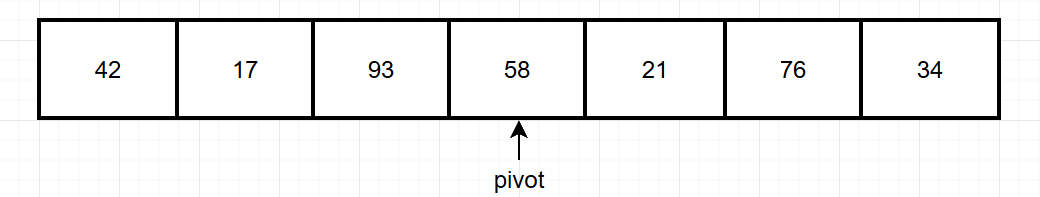
\includegraphics[width=0.75\linewidth]{img/quick_sort/1.png}
\end{figure}

\begin{enumerate}
    \item Trước tiên ta chọn $pivot = 58$ (phần tử ở giữa mảng) và tiến hành phân hoạch mảng thành hai phần:
    \begin{itemize}
        \item Phần bên trái chứa các phần tử nhỏ hơn hoặc bằng $58$: $[42, 17, 34, 21]$
        \item Phần bên phải chứa các phần tử lớn hơn $58$: $[93, 76]$
    \end{itemize}
    \item Ta sẽ di chuyển các phần tử sao cho các phần tử nhỏ hơn hoặc bằng $pivot$ sẽ nằm bên trái $pivot$ và các phần tử lớn hơn $pivot$ sẽ nằm bên phải $pivot$.
    
    \begin{figure}[H]
        \centering
        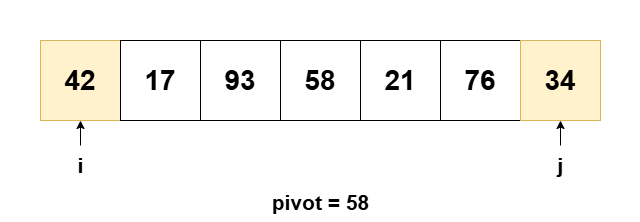
\includegraphics[width=0.75\linewidth]{img/quick_sort/2.png}
        
        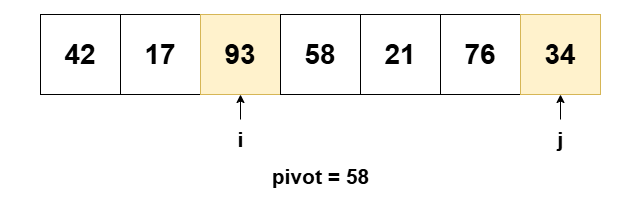
\includegraphics[width=0.75\linewidth]{img/quick_sort/3.png}
        
    \end{figure}
    
    \begin{figure}[H]
        \centering
        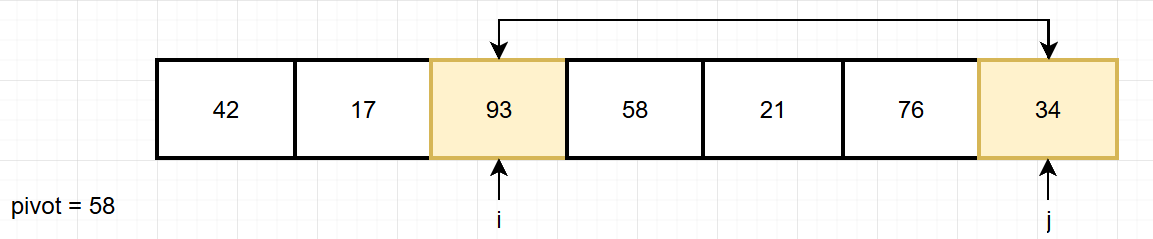
\includegraphics[width=0.75\linewidth]{img/quick_sort/4.png}
    
        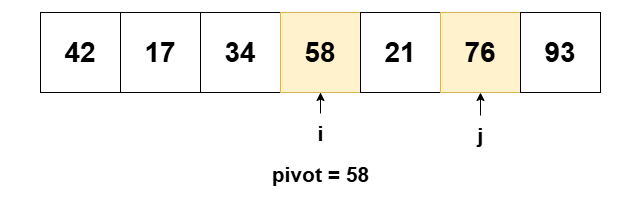
\includegraphics[width=0.75\linewidth]{img/quick_sort/5.png}
    
        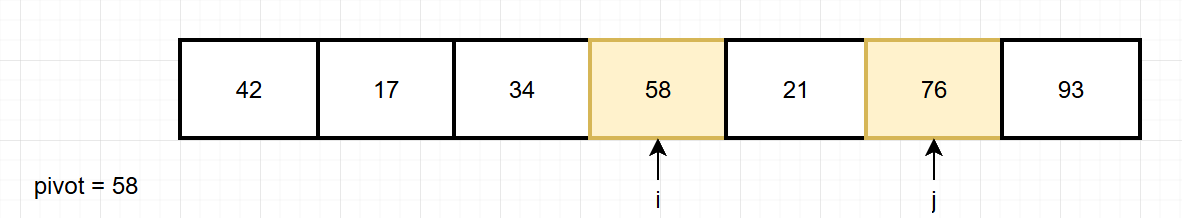
\includegraphics[width=0.75\linewidth]{img/quick_sort/6.png}
        
        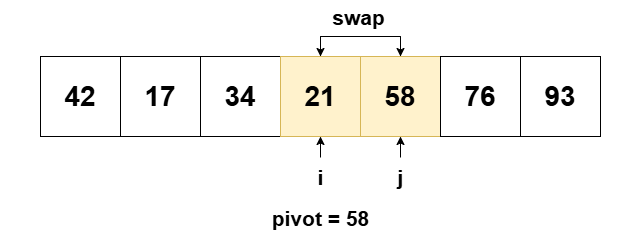
\includegraphics[width=0.75\linewidth]{img/quick_sort/7.png}
        
        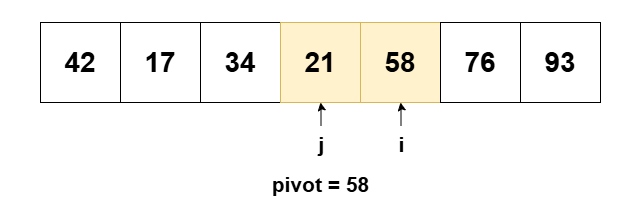
\includegraphics[width=0.75\linewidth]{img/quick_sort/8.png}
    \end{figure}

    \item Đến đây ta gọi đệ quy cho hai phần mảng mới được phân hoạch là $[42, 17, 34, 21]$, $[58, 76, 93]$ và cứ tiếp tục như vậy cho đến khi ta không thể phân hoạch nhỏ hơn được nữa.
    \begin{figure}[H]
        \centering
        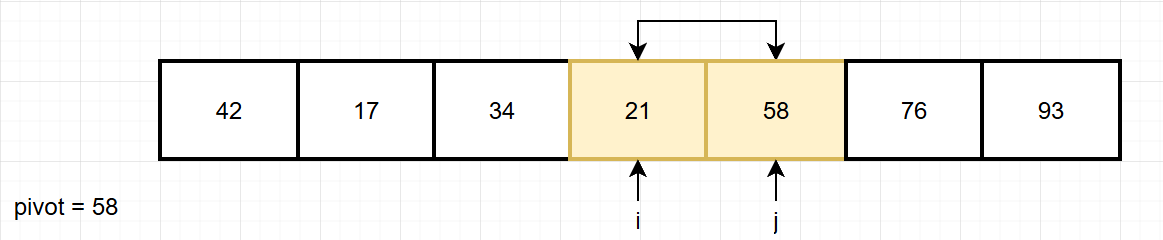
\includegraphics[width=1\linewidth]{img/quick_sort/9.png}
        
    \end{figure}

    \item Sau khi thực hiện tất cả bước trên ta sẽ thu được mảng đã được sắp xếp.
    \begin{figure}[H]
        \centering
        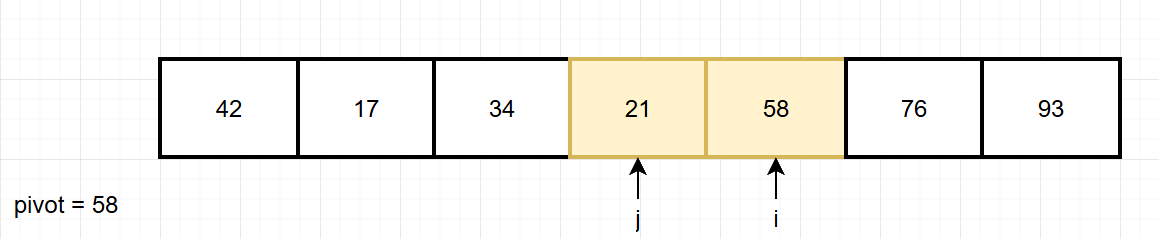
\includegraphics[width=0.75\linewidth]{img/quick_sort/10.png}
    \end{figure}
\end{enumerate}

\subsubsection{Độ phức tạp} 
\begin{itemize}
    \item[\textbf{--}]\textbf{Thời gian:}
        \begin{itemize}
            \item[$\bullet$] \textbf{Best Case:} $\mathcal{O}(n \cdot \log{}n)$, xảy ra khi việc chọn \textit{pivot} có thể phân hoạch thành 2 phần đều nhau.
            \item[$\bullet$] \textbf{Average Case:}  $\mathcal{O}(n \cdot \log{}n)$, thời gian chạy trung bình của \textit{Quick sort} thường gần với trường hợp tốt nhất hơn là trường hợp tệ nhất. \cite{CLRS2009} 
            \item[$\bullet$] \textbf{Worst Case:}  $\mathcal{O}(n^{2})$, xảy ra khi việc chọn \textit{pivot} không thể phân hoạch mảng thành 2 phần đều nhau, chẳng hạn một bên có 1 phần tử và bên còn lại có $n - 1$ phần tử.
        \end{itemize}
    \item[\textbf{--}]\textbf{Không gian:} phụ thuộc vào độ sâu ngăn xếp của việc gọi đệ quy. Cụ thể:
        \begin{itemize}
            \item[$\bullet$] \textbf{Best Case:} $\mathcal{O}(\log{}n)$, khi việc phân hoạch mảng thành 2 phần đều nhau dẫn đến độ sâu ngăn xếp của việc gọi đệ quy là $\log{}n$.
            \item[$\bullet$] \textbf{Worst case:} $\mathcal{O}(n)$, khi việc phân hoạch mảng thành 2 phần bị lệch dẫn đến độ sâu ngăn xếp của việc gọi đệ quy có thể đạt tới $n$. 
            \item[$\bullet$] \textbf{Auxiliary space:} \textit{Quick sort} là thuật toán \textit{in-place}, chỉ thay đổi vị trí các phần tử trong mảng.
        \end{itemize}
    \item[\textbf{--}]\textbf{Tính ổn định:} Không ổn định vì nó không đảm bảo vị trí ban đầu của các phần tử bằng nhau trong quá trình sắp xếp.
\end{itemize}